\documentclass[10pt]{article}
\usepackage[utf8]{inputenc}
\usepackage[czech]{babel}
\usepackage{a4wide}

\usepackage{graphicx}


\newcommand{\labtitle}[4]{
	\begin{titlepage}
		\begin{center}
			\mbox{} \\[4cm]
			{\huge {#1}} \\[2cm]
			{\Large #2}  % \\[.2cm]
			{\large #3 } \\[.7cm]
			{\normalsize měřeno #4}
		\end{center}
	\end{titlepage}
}


\begin{document}

% -- title page -- %
\labtitle{Rezonanční obvod}
 {Tomáš Maršálek}
 {(A10B0632P)}
 {17.\,října 2011}
% -- title page -- %


\section{Měřící potřeby a přístroje}
nízkofrekvenční generátor, nízkofrekvenční milivoltmetr, RLC měřič, 
panel s cívkou, kondenzátorem a třemi odpory

\section{Naměřené hodnoty}

\begin{minipage}[t]{0.5\textwidth}
\begin{flushleft}
Hodnoty součástek  \\[.2cm]
\begin{tabular}[b]{|cc|c|}
\hline
$R_1$ & $[k\Omega]$ & 9.68 \\
\hline
$R_2$ & $[k\Omega]$ & 5.30 \\
\hline
$R_3$ & $[k\Omega]$ & 1.82 \\
\hline
$R_0$ & $[\Omega]$  & 50   \\
\hline
$R_L$ & $[k\Omega]$ & 1.6  \\
\hline
$C_i$ & $[pF]$      & 114  \\
\hline
$C$ & $[nF]$        & 13.1 \\
\hline
$L$ & $[H]$         & 4.42 \\
\hline
\end{tabular} \\
\end{flushleft}
\end{minipage}
\begin{minipage}[t]{0.45\textwidth}
\begin{flushright}

Napětí při změně frekvence \\[.2cm]

\begin{tabular}{|c|c|c|c|c|c|} \hline
$R_1$ & $U_c$ & $R_2$ & $U_c$ & $R_3$ & $U_c$ \\
\hline
70 & 1.5 & 70 & 1.4 & 70 & 1.4 \\
122 & 1.5 & 118 & 1.4 & 108 & 1.4 \\
174 & 1.5 & 169 & 1.5 & 158 & 1.4 \\
221 & 1.6 & 225 & 1.6 & 209 & 1.6 \\
271 & 1.7 & 265 & 1.6 & 259 & 1.6 \\
320 & 1.8 & 322 & 1.8 & 314 & 1.8 \\
373 & 1.9 & 373 & 2.0 & 352 & 2.0 \\
421 & 2.0 & 425 & 2.2 & 409 & 2.2 \\
467 & 2.2 & 469 & 2.4 & 451 & 2.6 \\
525 & 2.3 & 529 & 2.9 & 511 & 3.2 \\
572 & 2.3 & 574 & 3.2 & 558 & 4.2 \\
619 & 2.3 & 618 & 3.4 & 600 & 5.4 \\
670 & 2.2 & 670 & 3.2 & 652 & 6.2 \\
715 & 2.0 & 727 & 2.7 & 723 & 4.2 \\
780 & 1.7 & 768 & 2.3 & 749 & 3.5 \\
840 & 1.4 & 819 & 1.8 & 805 & 2.4 \\
923 & 1.1 & 947 & 1.0 & 941 & 1.2 \\
998 & 0.9 & 1051 & 0.8 & 1020 & 0.9 \\
1090 & 0.7 & 1111 & 0.6 & 1101 & 0.7 \\
1190 & 0.5 & 1191 & 0.5 & 1192 & 0.5 \\
\hline
\end{tabular}

\end{flushright}
\end{minipage}



\section{Výpočty}
Pomocí vzorce pro rezonanční úhlovou frekvenci v elektrickém obvodu
\begin{equation}
w_{rez} = \sqrt{\frac{1}{LC} - \frac{R^2}{2L^2}}
\end{equation}

\noindent
a vzorce pro konstantu útlumu
\begin{equation}
b = \frac{R}{2L}
\end{equation}

\noindent
vypočteme tyto hodnoty pro všechny tři odpory. Celkový odpor $R$ je součtem
odporů všech součástek. \\
\begin{equation}
R = R_0 + R_i + R_L~~ pro~i \in \{1, 2, 3\}
\end{equation}

\noindent
Obvod beze ztrát ($R = 0$) by měl rezonanční úhlovou frekvenci 
\begin{equation}
w_{rez} = \sqrt{\frac{1}{LC}}
\end{equation}

\noindent
Výsledné frekvence pak z úhlových určíme ze vztahu
\begin{equation}
f_{rez} = \frac{w_{rez}}{2 \pi}
\end{equation}


\begin{tabular}[b]{|l|c|c|c|c|}
\hline
& celkový odpor [$k \Omega$] & konstanta útlumu & rezonanční frekvence [Hz] & 
                   $f_{max}$ [Hz] \\
\hline
$R_1$ & 11.33 & 1281.7 & 592.38 & 572 \\
$R_2$ & 6.95  & 786.2  & 634.70 & 618 \\
$R_3$ & 3.47  & 392.5  & 652.95 & 652 \\
$beze~ztr\acute{a}t$  & 0 & 0 & 658.90 & - \\
\hline
\end{tabular}

\vspace{1cm}

\includegraphics[width=10cm,angle=270]{graf.eps}

\section{Závěr} 
Naměřené hodnoty odpovídají vypočítaným. Pro vyšší přesnost by
bylo možné snížit interval mezi po sobě následujícími frekvencemi při měření,
ale z časových důvodů to nebylo možné.

\end{document}
